
Notre étude se limite, en terme de périmètre fonctionnel, à l'activité de Maintenance de la société SPIE Sud-Est. Les deux sections suivantes apportent des précisions sur cette société.

\section{Présentation générale de SPIE Sud-Est}

SPIE Sud-Est est une filiale régionale de services multitechniques de SPIE Opérations sur le quart sud-est de la France.

\begin{figure}[H]
    \label{fig-LABEL-DE-LA-FIGURE}
    \noindent\makebox[\textwidth]{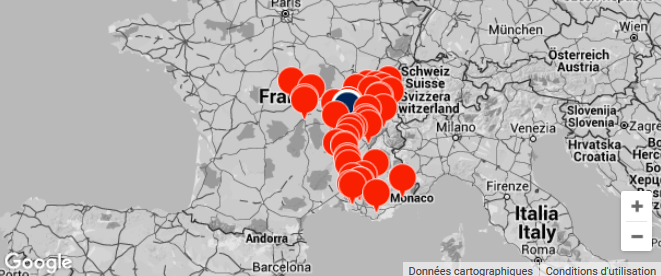
\includegraphics[width=10cm]{figures/implentations_spie.png}}
    \caption{Cartographie des implémentations de SPIE Sud-Est}
\end{figure}

Elle propose à ses clients un service de proximité et une offre diversifiée dans les domaines de l'énergie et des communications et les accompagne dans la conception, la réalisation, l’exploitation et la maintenance d’installations économes en énergie et respectueuses de l’environnement

\section{Organisation géographique et métiers de SPIE Sud-Est}

Du point de vue de l'organisation géographique, la société SPIE Sud-Est est organisée en territoires qui sont parmis les suivants : \\
\begin{itemize}
    \item[\textbullet] Rhône Alpes Auvergne
    \item[\textbullet] Espace Lémanique
    \item[\textbullet] Grand Dauphiné
    \item[\textbullet] Provence Alpes Côte d'Azur\\
\end{itemize}
    
La société SPIE Sud-Est remplit des missions dans les secteurs suivants :  \\
\begin{itemize}
    \item[\textbullet] Maintenance tertiaire
    \item[\textbullet] Génie climatique
    \item[\textbullet] Services aux industries
    \item[\textbullet] Télécoms services
    \item[\textbullet] Infrastructure / énergie \& transport
\end{itemize}